\documentclass{beamer}

\usepackage{lmodern}
\usepackage{attrib}
\usepackage{verse}
\usepackage{altverse}
\usepackage{bibleref}
\usepackage{multicol}

%\graphicspath{graphics/}
\setbeamercolor{frametitle}{fg=black}
%\setbeamertemplate{frametitle}{
%    \vspace{0.5cm}
%    \insertframetitle
%}

\title{Having a Heart Like Jesus}
%\subtitle{The Life Of Jesus}
%\author[WSCOC]{Walnut Street Church of Christ}
\date{March, 2014}

\AtBeginSection[]
{
\begin{frame}
\frametitle{\insertlecture}
\tableofcontents[currentsection]
\end{frame}
}

%\includeonlylecture{March 02}
%\includeonlylecture{March 09}
\includeonlylecture{March 16}

\begin{document}
\frame{\titlepage}


\begin{frame}
\frametitle{We all need constant attitude adjustments.}
Seven of the nine beatitudes focus on the condition of our heart.\\~\\
\begin{quote}
For the word of God is living and active, sharper than any two-edged sword, piercing to the division of soul and of spirit, of joints and of marrow, and \textbf{discerning the thoughts and intentions of the heart}.

\attrib{\bibleverse{Heb}(4:12), ESV}
\end{quote}

% I don't like this one
%\begin{quote}
%What I am eager for is that all the Christians there will be filled with \textbf{love that comes from pure hearts},and that their minds will be clean and their faith strong.

%\attrib{\bibleverse{ITim}(1:5), TLB}
%\end{quote}
\end{frame}

\lecture{The Poor in Spirit Need Jesus}{March 02}
\lecture{The Poor in Spirit Need Jesus}{March 02}
\begin{frame}

\frametitle{What are you really saying when \dots}
\begin{columns}
\column{4.5cm}
you complain about\\things at church,\\~\\

you think others are\\less spiritual than you,\\~\\

you cannot let go\\after someone hurts you.\\~\\ 

you are more merciful to\\yourself than to others\dots\\~\\~\\
\centering\uncover<2->{\alert{``I deserve to be here.''}}
\column{5.5cm}
\uncover<2->{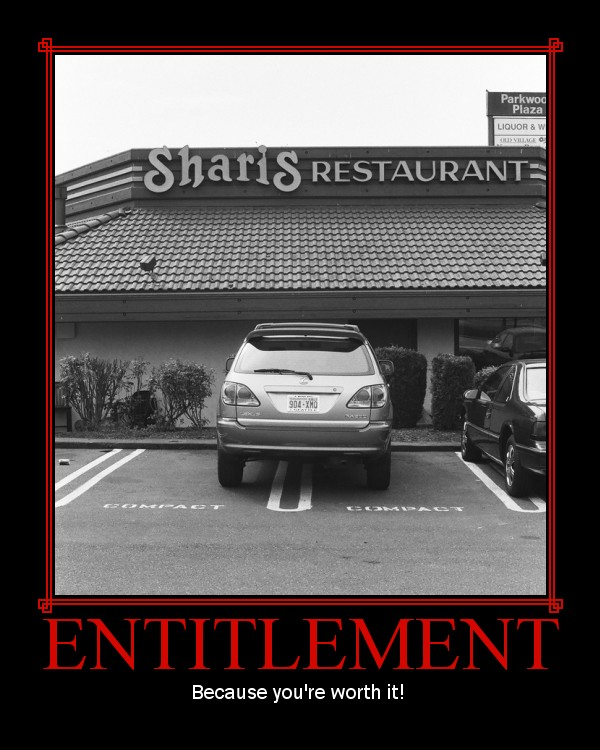
\includegraphics[width=\textwidth]{graphics/entitlement.jpg}}
\end{columns}
~\\
\end{frame}


\begin{frame}
\frametitle{This week's readings remind us that\\we are all sinners.}

Peter recognizes his sinfulness\\~\\
Jesus forgives the sins of a paralytic man.\\~\\
Jesus call Matthew, a sinner who wants to repent.


\end{frame}

\begin{frame}
\frametitle{When we remember our sinfulness,\\we realize  our dependence on Jesus.}
\begin{verse}
Blessed are the poor in spirit,\\for theirs is the kingdom of heaven.

Blessed are those who mourn,\\for they shall be comforted.

Blessed are the meek,\\for they shall inherit the earth.

\attrib{\bibleverse{Matthew}(5:3-5)}
\end{verse}
\end{frame}

\begin{frame}
\frametitle{\insertlecture}
\tableofcontents[sectionstyle=show/show]
\end{frame}

\section{We do not deserve to be in the presence of Jesus.}
\begin{frame}
\frametitle{Peter knows what kind of person he is.}
\framesubtitle{\bibleverse{Luke}(5:1-11)}

\begin{columns}
\column{4.5cm}
He hears Jesus teach\\of the kingdom.\\~\\
He sees Jesus perform a personally relevant miracle.\\~\\
The miracle produces belief --- and guilt.\\~\\
\column{6cm}
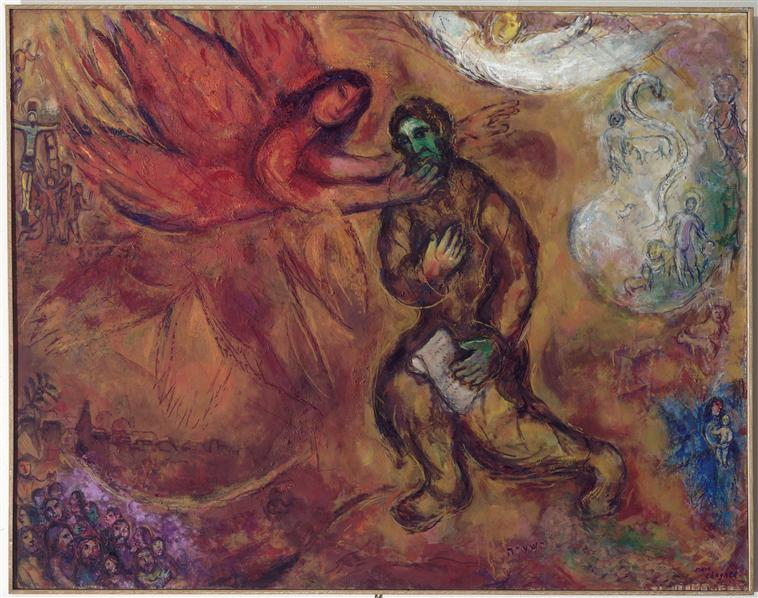
\includegraphics[width=\textwidth]{graphics/prophet-isaiah-1968.jpg}\\
\tiny{A similar event happened to Isaiah.}\\~\\
%\raggedleft\tiny{Prophet Isaiah, Marc Chagall, 1968}
\end{columns}
\begin{quote}
When Simon Peter saw what had happened,\\he bowed down before Jesus and said,\\``Go away from me, Lord. I am a sinful man!''

\attrib{\bibleverse{Luke}(5:8), NCV}
\end{quote}
\end{frame}

\begin{frame}
\frametitle{The gospel is a better mirror than a bat.}
\begin{columns}
\column{5cm}
Do not make the sins of others\\too big.\\~\\
Do not make your own sins\\too small.\\~\\~\\
\column{5cm}
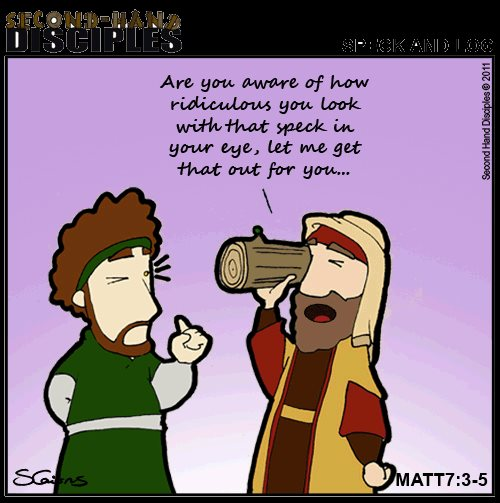
\includegraphics[width=\textwidth]{graphics/beam.jpg}\\
\end{columns}
~\\Peter probably was a horrible person.\\
But, Jesus could transform him.
\end{frame}

\section{But, Jesus is the only one with power to forgive us.}
\begin{frame}
\frametitle{Jesus heals a paralytic physically and spiritually.}
\framesubtitle{\bibleverse{Mark}(2:1-12)}
\begin{columns}
\column{5.5cm}
The paralytic has some\\unashamed friends.\\~\\
It is `their' faith that\\prompts the Lord to forgive.\\~\\
\column{4.5cm}
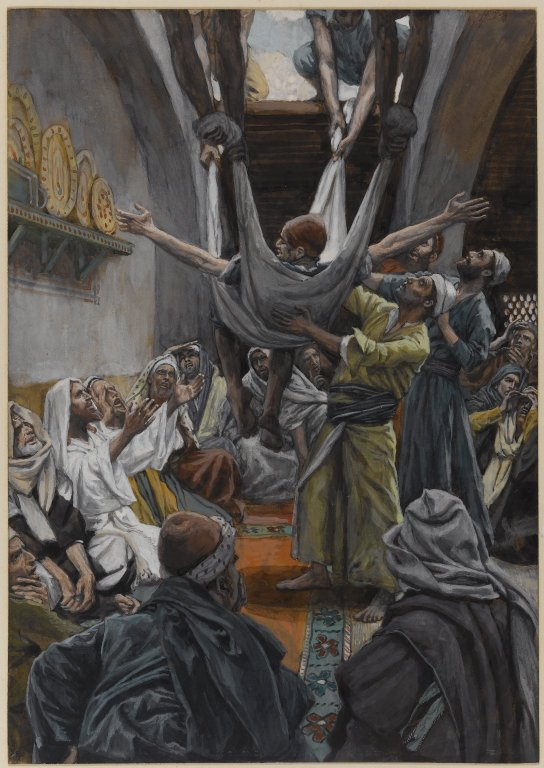
\includegraphics[width=\textwidth]{graphics/paralytic.jpg}
\end{columns}
\centering~\\
Jesus has the power to grant \emph{everything} man needs.
\end{frame}

\begin{frame}
\frametitle{Where else can you go for forgiveness but to Jesus?}
\begin{quote} 
And when Jesus saw \textbf{their faith}, he said to the paralytic, ``Son, \textbf{your sins are forgiven}.''

\attrib{\bibleverse{Mark}(2:5)}
\end{quote}

\begin{quote}
Is anyone among you sick? Let him call for the elders of the church, and let them pray over him, anointing him with oil in the name of the Lord. And \textbf{the prayer of faith will save the one who is sick, and the Lord will raise him up. And if he has committed sins, he will be forgiven}. Therefore, confess your sins to one another and pray for one another, that you may be healed. The prayer of a righteous person has great power as it is working.

\attrib{\bibleverse{James}(5:14-16)}
\end{quote}

\end{frame}

\section{So, He comes to those who want forgiveness.}

\begin{frame}
\frametitle{The healthy don't need a doctor, but the sick do.}
\framesubtitle{\bibleverse{Luke}(5:27-39)}
Jesus befriends Matthew and his cohort of tax collectors.\\~\\
Jesus wants those \emph{sinners} to become \emph{repenters}.\\~\\
The Pharisees have a totally different world-view\\where the righteous and the sinner never change.
\end{frame}

\begin{frame}
\frametitle{Christians are defined by their willingness to change.}
Old wineskins are tough and unyielding.\\
New wineskins are receptive to God's teachings.\\
Christians must \emph{live} as new wineskins.\\~\\~\\
This principle can be applied every time we come together.
\begin{itemize}
\item Study is not just about confirmation. It's about learning.
\item Resist the urge to shoot someone's thought down immediately.
\item Every generation has to interpret the Bible for themselves.
\end{itemize}

\end{frame}

\section*{Conclusion}
\begin{frame}
\frametitle{}
Know who you are\ldots\\
A sinner, forgiven.\\~\\
Be willing to change\ldots\\
by Jesus' power.

\end{frame}

\section*{Tough Passages}

\begin{frame}
\begin{quote}
\dots And the power of the Lord was with him to heal \dots

\attrib{\bibleverse{Luke}(5:17b)}
\end{quote}

\end{frame}


\lecture{I Require Mercy and Not Sacrifice}{March 09}
\begin{frame}
\frametitle{Attention Getter}
something
\end{frame}

\begin{frame}
\frametitle{Need}
some bible verses
\end{frame}

\begin{frame}
\frametitle{task}
current reading
\end{frame}

\begin{frame}
\frametitle{Solution in short}
\end{frame}

\begin{frame}
\frametitle{\insertlecture}
\tableofcontents[sectionstyle=show/show]
\end{frame}

\section{The Sabbath was for man's good}
\begin{frame}
\frametitle{Man healed at pools of Bethesda}
Man is healed at the pools of Bethesda 
\end{frame}

\begin{frame}
\frametitle{}
\end{frame}

\section{Jesus is Lord of the Sabbath}

\begin{frame}
\frametitle{Disciples pick grain on the Sabbath}
\end{frame}

\begin{frame}
\frametitle{Situation Ethics}
\end{frame}

\section{God's law does good.}

\begin{frame}
\frametitle{Man's hand healed on the Sabbath}
\end{frame}

\begin{frame}
\frametitle{Sometimes we do nothing because we're afraid of doing something wrong}
\end{frame}

\section*{Conclusion}
\begin{frame}
\frametitle{Be merciful}
\end{frame}

\section*{Tough Passages}
\begin{frame}
\frametitle{Some newer translations leave out \bibleverse{John}(5:4)}
\framesubtitle{For example: ESV, NIV}

\footnotesize  
\begin{quote}
\textsuperscript{3} In these lay a great multitude of impotent folk, of blind, halt, withered, \textbf{waiting for the moving of the water. \textsuperscript{4} For an angel went down at a certain season into the pool, and troubled the water: whosoever then first after the troubling of the water stepped in was made whole of whatsoever disease he had.} \textsuperscript{5} And a certain man was there, which had an infirmity thirty and eight years.

\attrib{\bibleverse{John}(5:3-5), KJV}
\end{quote}
\normalsize 
Newer translations are probably right for the following reasons.
\begin{itemize}
\item KJV is from the \textit{Textus Recepticus} whose compiled manuscripts date from 1100 A.D. or later.
\item No manuscripts prior to 500 A.D. contains verse 4.
\item Multiple Greek manuscripts around 900 A.D. have marks questioning the validity of this verse.
\item The verse has multiple words occurring nowhere else in John.
\item The verse has a large number of variants in manuscripts.
\end{itemize}

\end{frame}


\lecture{Sermon on the Mount Part}{March 16}
%!TEX root = lifeOfJesus_AdultClass_201403_presentation.tex
\note{
Summary of Chapters 5 - 6 
If you're heart is not right, then you're not right.

You should not teach the sermon on the mount.  You should simply read it and let the lessons sink in.

Should I hit the highlights, hit the verses we get wrong or do a summary?

Really what I would like for people to learn from class is to meditate on how to do these things.  It's funny, we come up with all sorts of ways to accomplish goals as if the Bible is sort of incomplete when it comes to doing things.  And, in a way, we have to figure out what areas of our life apply to the lessons we're learning.
Some places the sermon on the mount tells you just how to do stuff.  In other places it's a little more vague.


5:13-16 Salt and Light.
5:17-20 This is the way that God has always wanted us to be.
5:21-32 When applying the Lord's commands, you have to think about the state of the heart that God is trying to get you to have.  Let's have some other examples.
5:38-end We have a different standard of living.
6:1-18 Down to earth person.  Your outside and your inside match. 
6:19-34 Priorities

The Beatitudes really contrast with how you might try to find happiness if you weren't taught by Jesus
How to be happy

They surround themselves with happy people
The cultivate resilience
They try to be happy
They are mindful of the good
They appreciate simple pleasures
They devote some of their time to giving
They let themselves lose track of time
They nix the small talk for deeper conversation
They make a point to listen
They uphold in-person connections
They look on the bright side

1 Be Proactive
2 Begin With The End in Mind
3 Put First Things First
4 Think Win/WIn
5 Seek First to Understand, THen to be Understood
6 Synergize
7 Sharpen the Saw

You have to visualize what you want

You don't need to interpret it.  You just have to find ways to incorporate it.  You have to ask, ``Where does this apply to my life?'' 

Heaven is only for people that know they don't belong there.
grieve, not only for sin but just in general for the things that get you down in life, 
People who are humble don't get ahead in this world.  But, you can't buy the earth.
You're blessed when you get your inside world -- your mind and heart -- put right.  Then you'll see the working of God in your life.  You've learned to think how God thinks.

How is it that my good works cause others to give glory to God.  I think maybe because when you put something good in someones life, they have an opportunity to see God as being good to them.

Do Christ came to fulfill the Law first.


What is it about the things you get?
I think that you can't really take them independently.
I think there's a tendency to think about.  There are some Christians that are this.  And others that are good at meekness, and others that are good at being peacable.  But, they aren't independent.  These describe a whole person.
And to some degree these 
}

\begin{frame}
\frametitle{Background on Sermon the Mount}
This is \emph{the} sermon Jesus taught:\\
on the plain, on the mountain, everywhere.\\~\\

Jesus made the intent of Law clear to people,\\
and taught about the kingdom.\\\bibleverse{Matthew}(5:17-20)\\~\\

Jesus taught with authority.\\\bibleverse{Matthew}(7:28-29)
\end{frame}

\begin{frame}
\frametitle{\insertlecture}
\tableofcontents[sectionstyle=show/show]
\end{frame}

\section{How can I be happy?}

\begin{frame}
\frametitle{``Blessed''}
\framesubtitle{\bibleverse{Matthew}(5:2-11)}
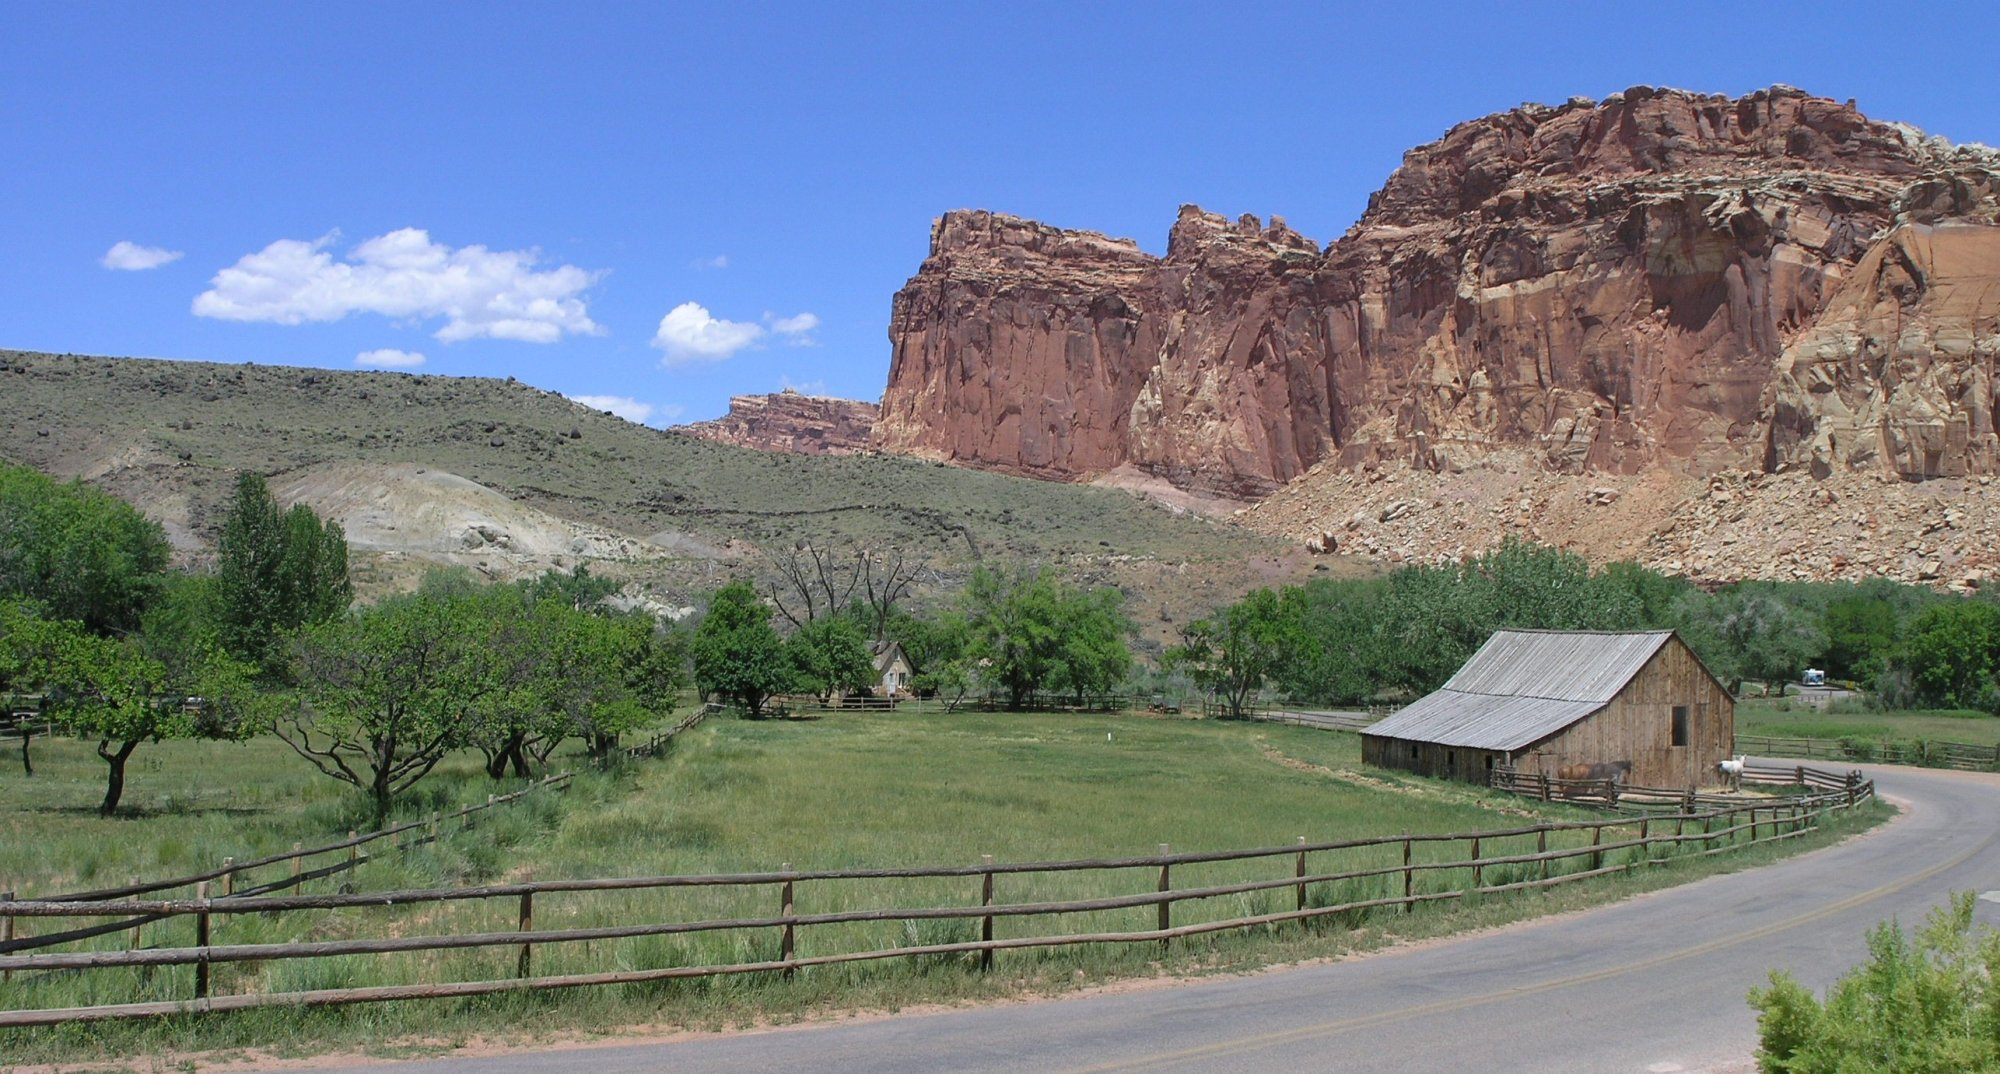
\includegraphics[width=\textwidth]{graphics/ranch.jpeg}
\end{frame}

\section{What's my purpose?}

\begin{frame}
\frametitle{Salt and Light}
\framesubtitle{\bibleverse{Matthew}(5:13-16)}
When our lives reflect God,\\perhaps others will see that God is good.
\end{frame}

\section{How do I know right from wong?}
\begin{frame}
\frametitle{Morality begins in the heart.}
\framesubtitle{\bibleverse{Matthew}(5:21-48)}
If your heart is not right, then you are not right. 

\end{frame}

\section{How do I keep my life in harmony?}
\begin{frame}
\frametitle{Christianity is about the whole person.}
\framesubtitle{\bibleverse{Matthew}(6:1-34)}
Christians want their outside and inside to look the same.
\end{frame}


\end{document}
